
\chapter{The Route Inspection/ Chinese Postman Problem}
\label{Appendix:ChinesePostman}


After solving the preceding ``pure'' version of the Eulerian-tour
problem---which seeks a tour of a graph which crosses each edge
precisely once---we discuss an extension of this problem which allows
us to augment a graph $\g$ by adding multiple edges between the same
two vertices.  (Terminologically, we thereby convert $\g$ to a {\it
  multi-graph} \index{multi-graph} \index{graph!multi-graph}
consisting of vertices and {\it multi-edges}.) \index{multi-edge} Not
obviously, adding multi-edges can often convert a graph $\g$ that does
not admit an Eulerian cycle into a multi-graph that does admit an
Eulerian cycle.  The problem of finding the {\em smallest} such
augmentation of $\g$---i.e., of adding the fewest multi-edges---is
called the \index{Route Inspection Problem} {\it Route Inspection
  Problem}; it is also often called the {\it Chinese Postman Problem},
\index{Chinese Postman Problem} in honor of its inventor, the Chinese
mathematician Kwan Mei-Ko \index{Kwan Mei-Ko} \cite{Kwan60}.



This section is devoted to studying the {\it Route Inspection
  Problem}, \index{Route Inspection Problem} also known as the {\it
  Chinese Postman Problem}, \index{Chinese Postman Problem} in honor
of its inventor, the Chinese mathematician Kwan Mei-Ko \index{Kwan
  Mei-Ko} \cite{Kwan60}.  This problem seeks to add as few multi-edges
\index{graph!multi-graph!multi-edge} as possible to a graph $\g$ in
order to render $\g$ Eulerian.  (A {\it multi-graph} is ``almost'' an
undirected graph.  It differs from a true graph because of the
possible presence of multiple multi-edges that connect the same two
vertices.)


We know from Proposition~\ref{thm:eulerian-cycle} in Section~\ref{sec:EulerianCycle} that if all of
$\g$'s vertices have even vertex-degrees, then---{\em and only then}---$\g$
admits an Eulerian cycle.  Therefore, in this case, {\em zero}
multi-edges need be added to $\g$ to render it Eulerian.  

Let us now present the more general problem of determining a cycle that contains all the edges in any graph, in particular when
there exist some odd vertices. From the previous section, we know that there is no Eulerian cycle in this case and thus, 
any feasible solution should duplicate some edges.
The problem is to duplicate the minimum.
This problem is known as the {\it chinese postman} and it is described below (in a french equivalent version).

A postman moved recently from Grenoble to a small village in the country side. 
He asked himself how to organize his daily tour by bike for distributing the letters in the shortest possible time. 
The director of the post office gives him the map and 
fortunately, the postman had some old souvenir of previous lectures in Graph Theory.  
The tour starts from the post office and of course, the postman has to go through every roads for distributing the letters before coming back
to his office.
The underlying graph is $G=(V,E)$ where $V$ is the (finite) set of cross points and $E$ is the set of the links between the cross roads
weighted by the distances.  

Fig.~\ref{fig:EulerianInitial} presents an example of the chinese postman problem. 
\begin{figure}[hbt]
\begin{center}
       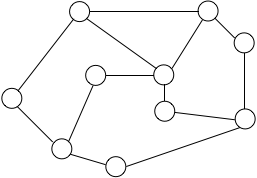
\includegraphics[scale=0.6]{FiguresGraph/EulerienInitial}
       \caption{An instance of the Chinese postman with $10$ cross-vertices.}
              \label{fig:EulerianInitial}
\end{center}
\end{figure}

\bigskip

This problem can be formulated mathematically in term of Eulerian
cycles.  Intuitively, the basic idea is to duplicate some edges that
are carefully chosen in order to use the previous construction of an
Eulerian tour of Section~\ref{sec:EulerianCycle} that will help the
postman to determine the optimal tour (of minimal length) using some
simple mathematical properties.
\bigskip

First, we know that there is an even number of odd vertices.
Considering the previous instance of the postman problem, there are $4$ such vertices (represented in grey in Fig.~\ref{fig:EulerianVodd}).

\begin{figure}[hbt]
\begin{center}
       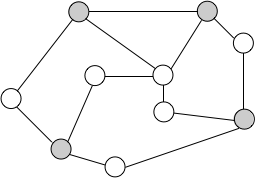
\includegraphics[scale=0.6]{FiguresGraph/EulerienVodd}
       \caption{The $4$ vertices with an odd degree in the previous instance.}
              \label{fig:EulerianVodd}
\end{center}
\end{figure}
\bigskip

As there exists a path between any pair of vertices of odd degree in $V_{odd}$,
we consider the complete graph whose vertices are the odd degree vertices weighting the edges with the shortest paths (denoted by $K_{odd}$).
As we mentioned in the preliminary properties, computing the shortest paths is a classical problem, which can be solved in polynomial time. 

\begin{figure}[hbt]
\begin{center}
       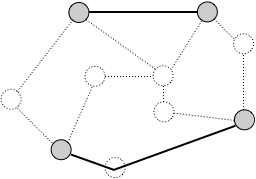
\includegraphics[scale=0.6]{FiguresGraph/EulerienPerfectMatching}
       \caption{The minimum weight perfect matching labelled by the shortest distances between the vertices of $V_{odd}$.}
              \label{fig:Eulerianperfectmatching}
\end{center}
\end{figure}
\bigskip

Then, it is possible to do the correspondence between the optimal solution of the postman problem and a perfect matching of minimal weight in $K_{odd}$
%Recall that a matching is a set of edges without common vertices. It is perfect if it has the maximum number of edges. 
by duplicating the edges of the minimal perfect matching.

\begin{figure}[hbt]
\begin{center}
       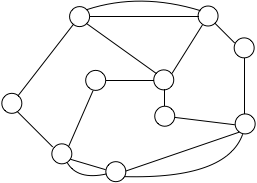
\includegraphics[scale=0.6]{FiguresGraph/EulerienFinal}
       \caption{Final step: adding the edges of the minimum perfect matching.}
              \label{fig:EulerianFinal}
\end{center}
\end{figure}

The main steps of the algorithm for determining the optimal tour are the following:

\begin{itemize}
\item Consider the complete graph with the odd vertices and compute its weight by the shortest paths.
Compute a perfect matching of minimal weight between these vertices. 
\item Duplicate all the edges along the paths of this matching.
\item Determine an Eulerian tour in this new graph with even degrees.
\end{itemize}

The optimality of this algorithm comes from the fact that the duplicated edges are the minimum possible ones.
% This is straightforward for two odd vertices.
Finally, all the vertices of the new graph are even since the degree of the odd vertices in $G$ is augmented by $1$
(extremities of the paths) and the other even vertices which are intermediate vertices of the paths remain even. 

\medskip

This short discussion is a good segu\'{e} to the material in the next
section, which led valuable perspective on our brief study of
Hamiltonian paths and cycles---and, indeed, on the computational
implications of that work.
